	Before proper testing could commence, covariances for the simulation had to be calculated from error measurements. This was done by measuring the error from the odometry topic, which in the simulation is the ground truth, to the various sensors over 400 samples while the bot traversed an arbitrary path. It should be noted that for the sensors that involve dead reckoning (Model, Joint, and IMU), the covariance in table \ref{tab:1} is calculated on the assumption that every measurement was based off an absolute reference. As dead reckoning techniques have the issue of accumulating error, the value shown would be incremental for every sample beyond the first.\par
	\begin{table}
	\centering
	\caption{Table of measured simulation covariances.}
	\label{tab:1}
	\begin{tabular}{ccc}
		\hline
		Sensor	&Measurement	&Covariance		\\\hline\hline
		Model		&x 			&$5.5*10^{-6}$	\\
		Model		&y			&$2.7*10^{-6}$	\\
		Model		&$\theta$		&$7.1*10^{-5}$	\\\hline\hline
		Joint		&x \& y		&$1.6*10^{-5}$	\\
		Joint		&$\theta$		&$7.2*10^{-5}$	\\\hline\hline
		IMU		&$\theta$		&$5.7*10^{-5}$	\\\hline\hline
		LiDAR		&x 			&$5.0*10^{-3}$	\\
		LiDAR		&y			&$5.0*10^{-3}$	\\
		LiDAR		&$\theta$		&$5.0*10^{-3}$	\\\hline
	\end{tabular}
	\end{table}
	
	Simulation performance was quite good for yaw, although a small error in yaw and a larger error in position can be seen when at faster velocities. The exact cause of this issue in simulation is still unknown. The physical LiDAR has a delay between each individual range measurement which would cause each measurements to be taken at different positions. This is not compensated for in the calculations, however, the simulation scan topic reports both scan time and time increment as 0.0 seconds. Meaning either the simulation does not publish these values as intended, or the range measurements are all taken simultaneously and the issue lies elsewhere.\par
	
	\begin{figure}
	    	\captionsetup{width=\columnwidth}
	   	\centering
	   	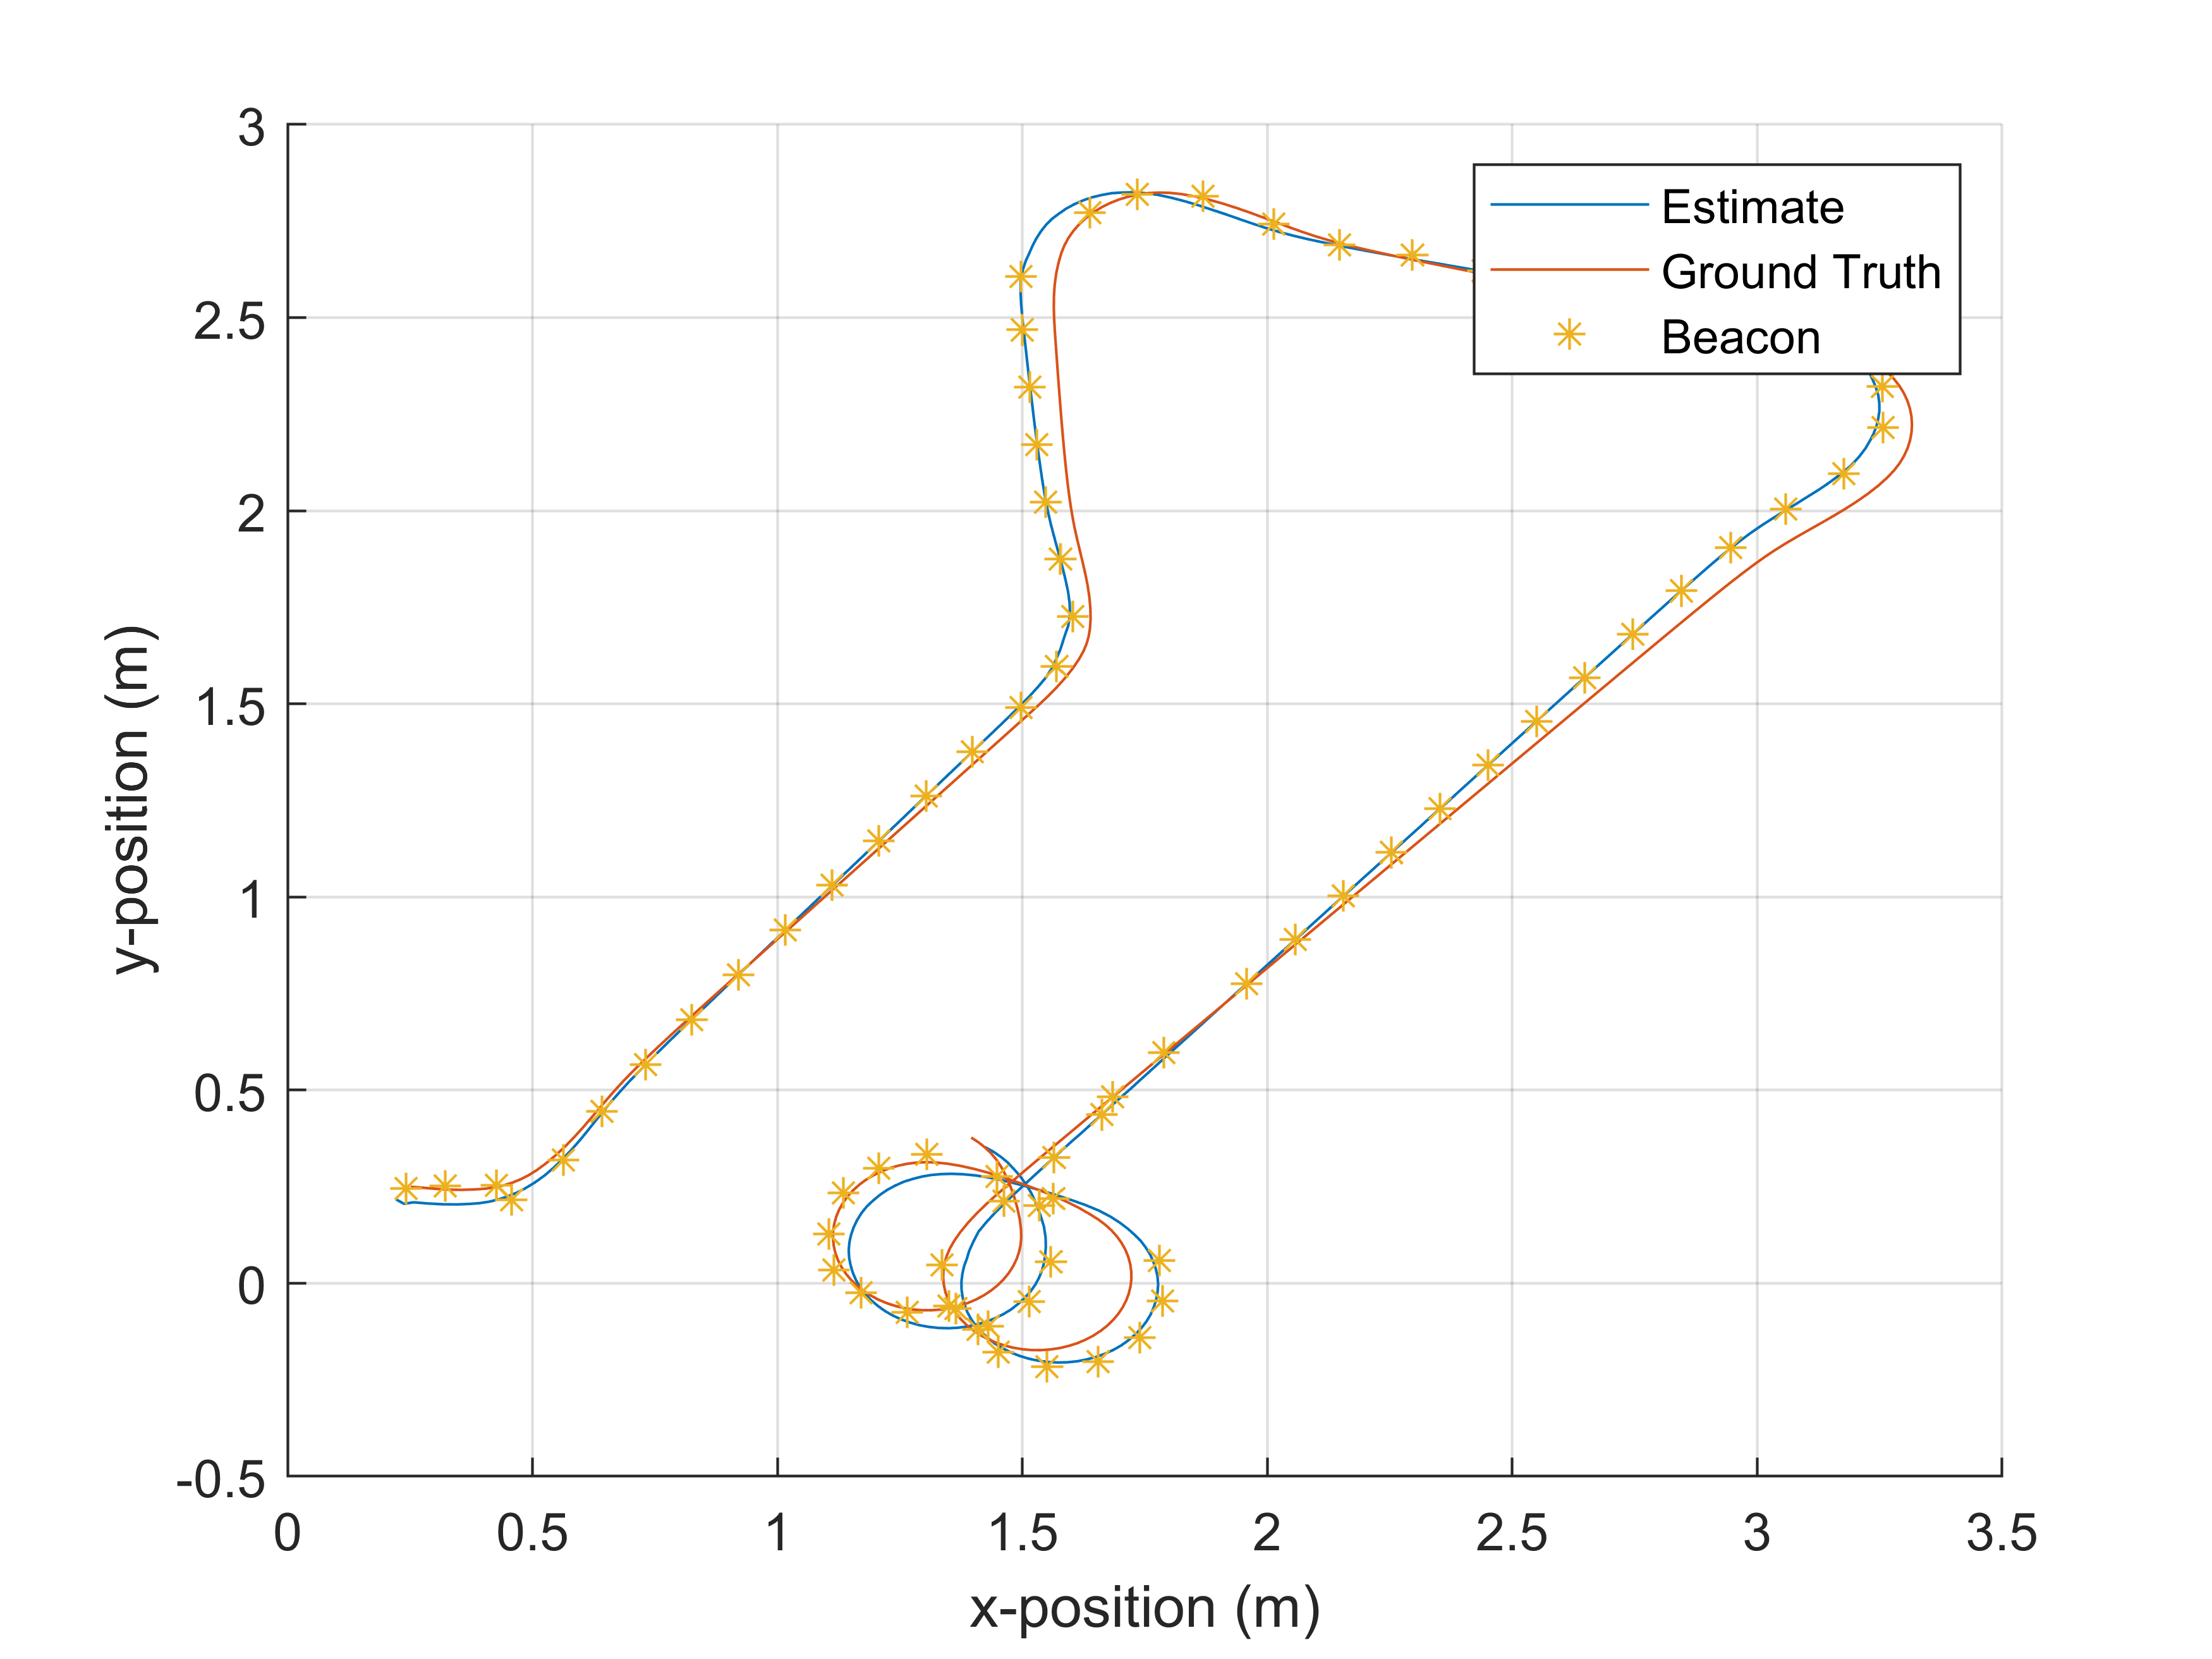
\includegraphics[width=\columnwidth]{./graphics/posSimu.png}
	   	\caption{Position estimates versus ground truth (Simulation).}
		\label{fig:pos}
	\end{figure}
	
	\begin{figure}
	    	\captionsetup{width=\columnwidth}
	   	\centering
	   	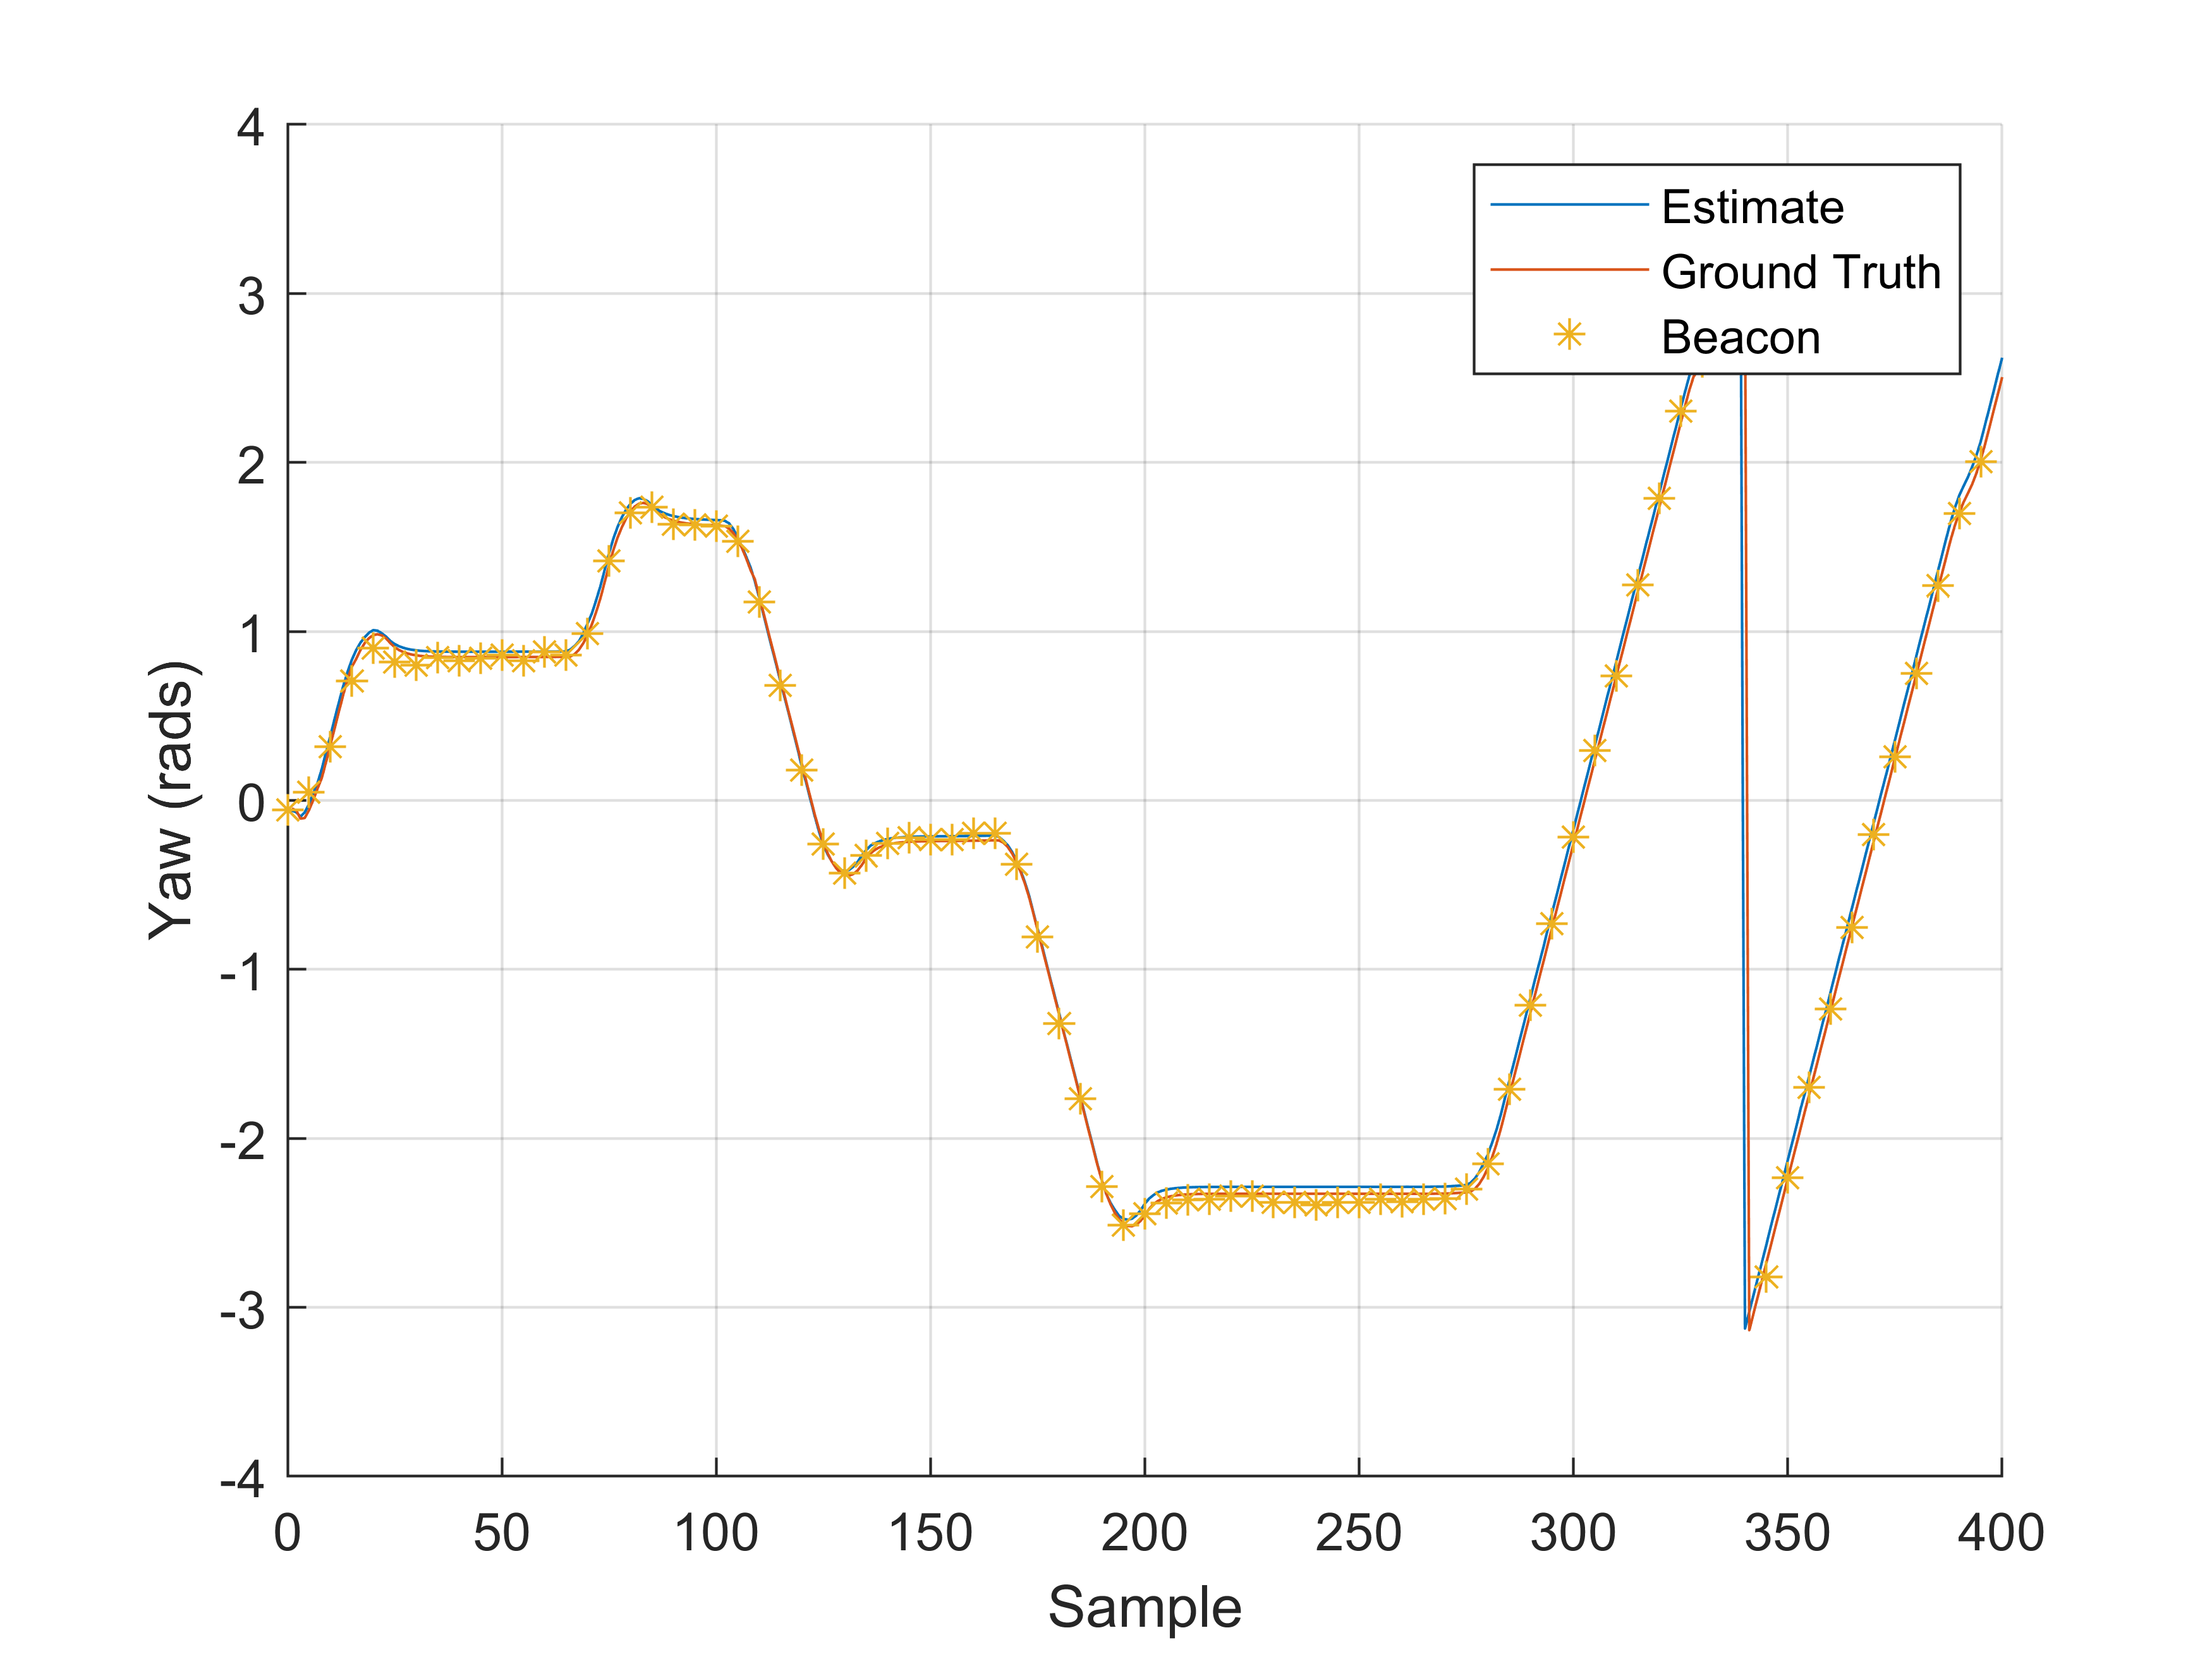
\includegraphics[width=\columnwidth]{./graphics/yawSimu.png}
	   	\caption{Yaw estimates versus ground truth (Simulation.}
		\label{fig:yaw}
	\end{figure}
	
	\begin{figure}
	    	\captionsetup{width=\columnwidth}
	   	\centering
	   	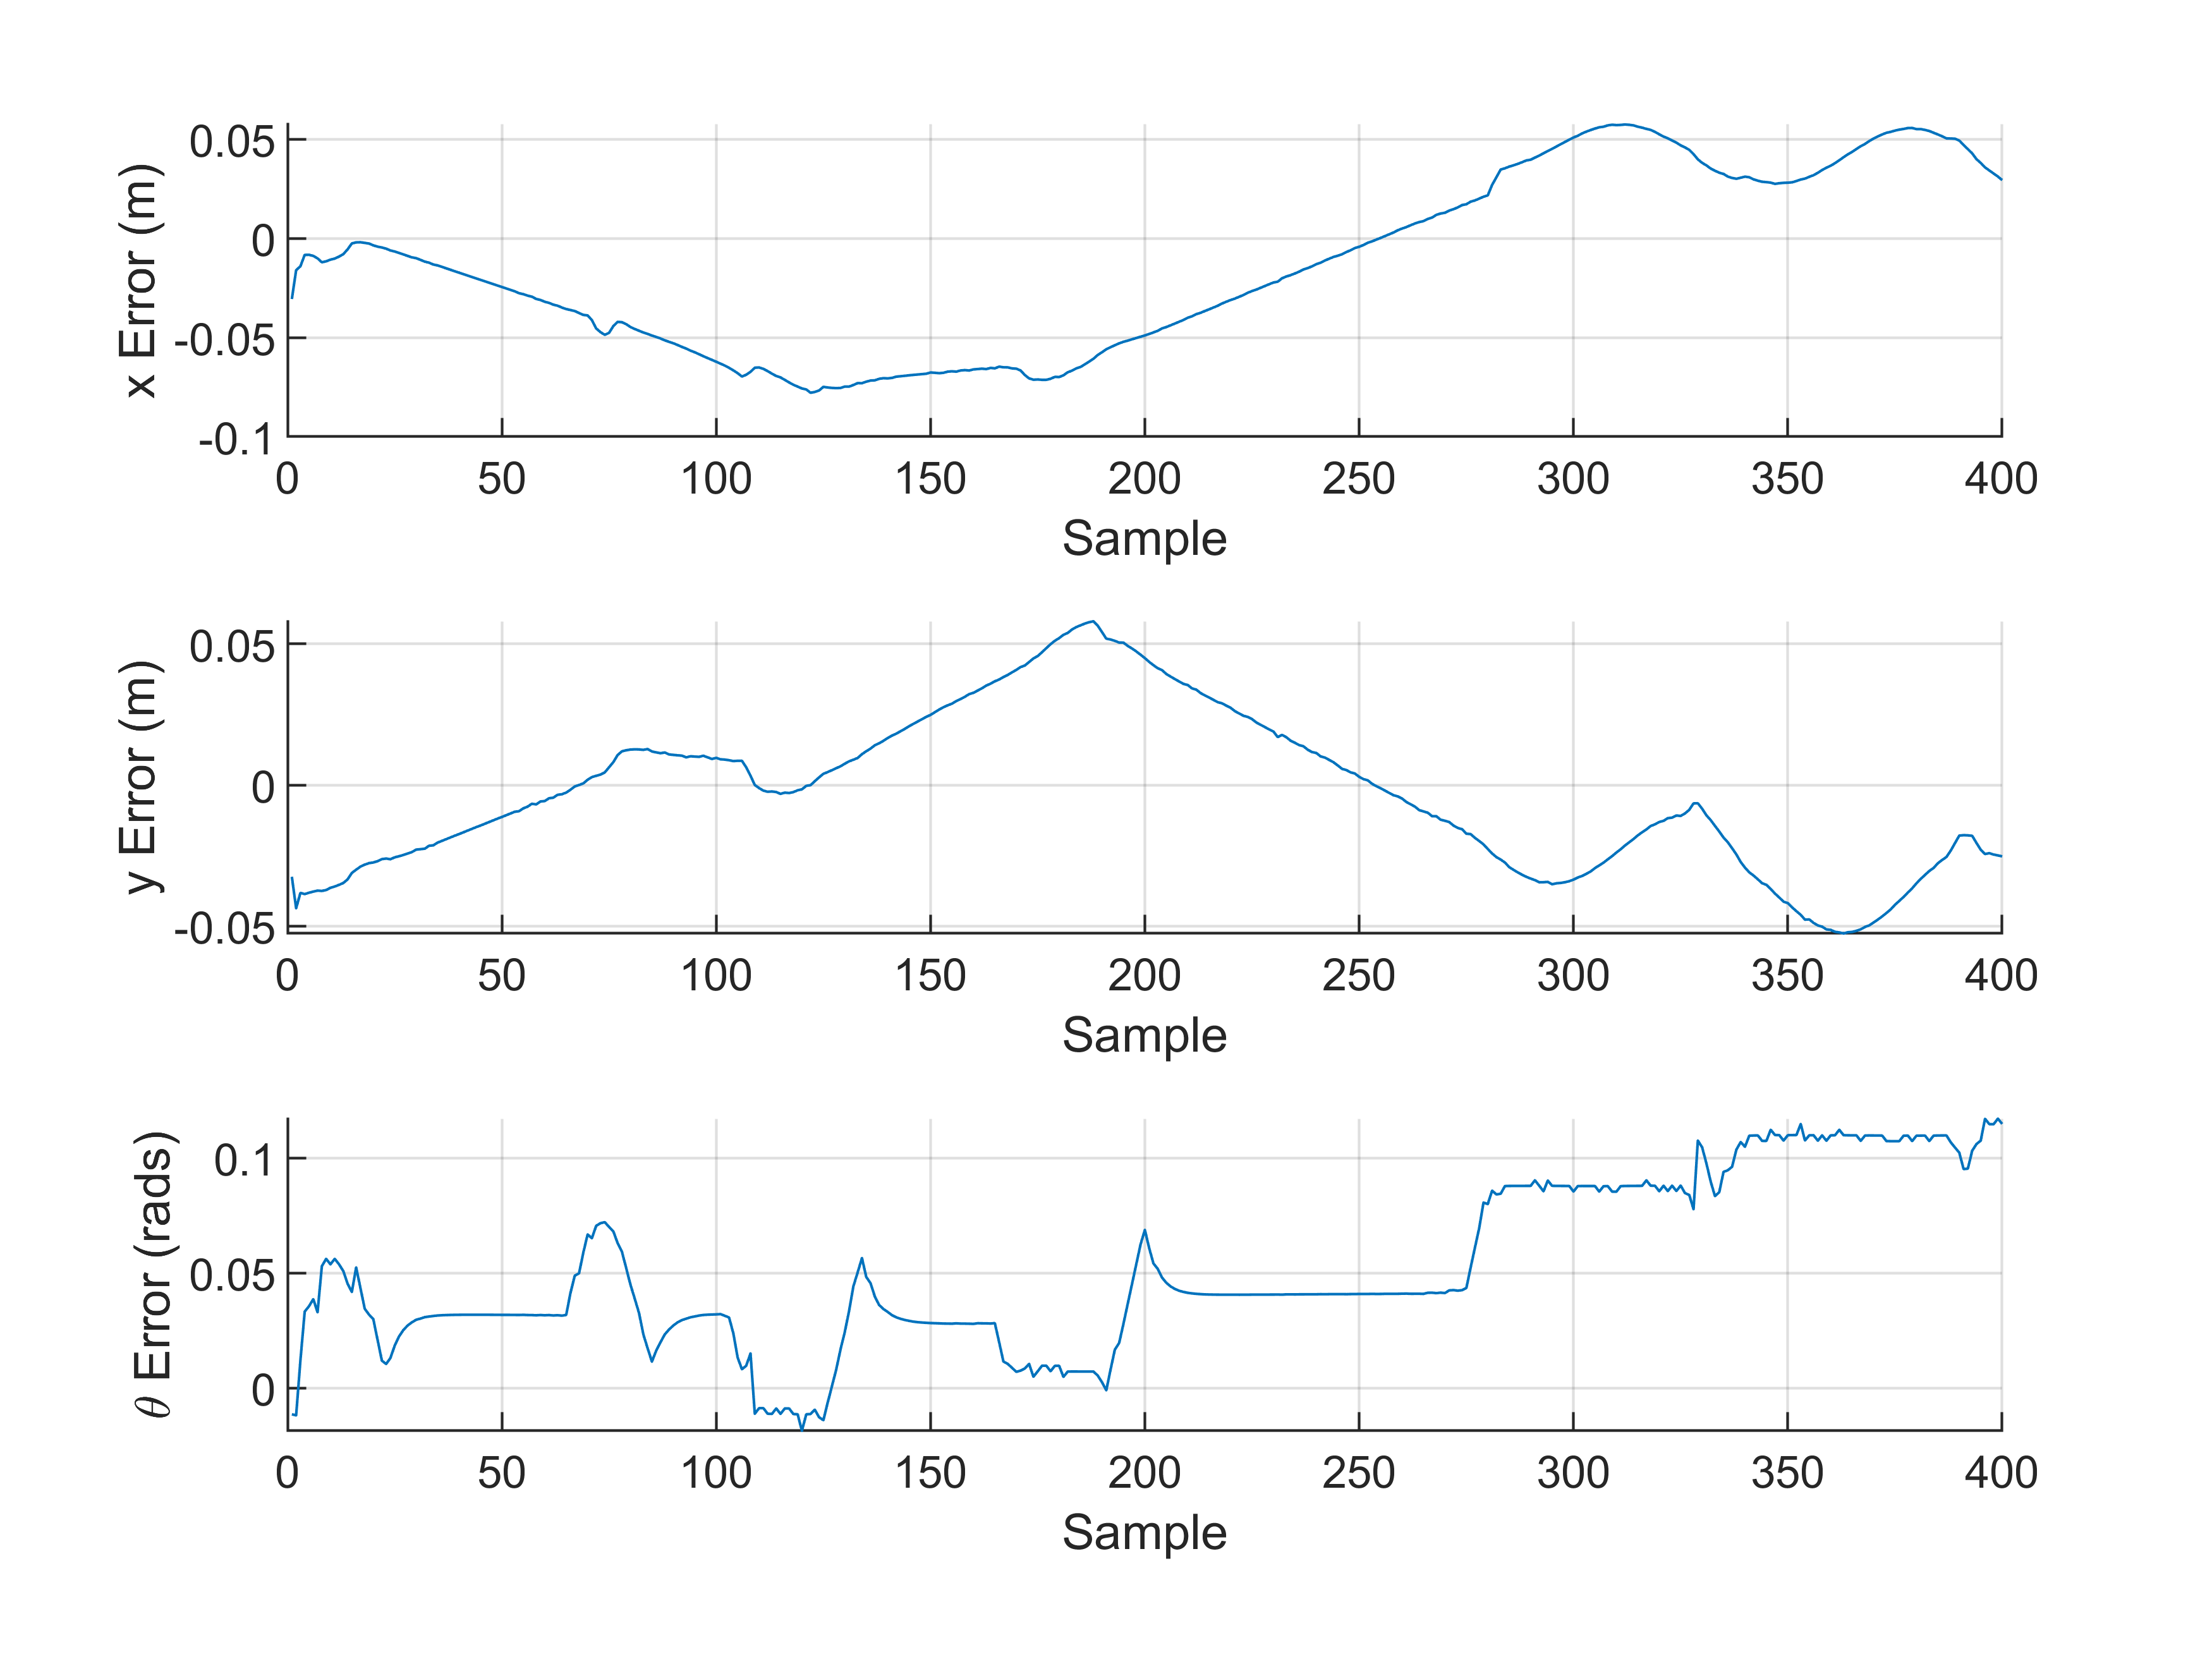
\includegraphics[width=\columnwidth]{./graphics/Error.png}
	   	\caption{Error plot of figure \ref{fig:pos} and \ref{fig:yaw}.}
		\label{fig:err2}
	\end{figure}
	
	
	Physical performance was acceptable considering the lack of controls. The field was not a perfect rectangle, the beacons that were used, though cylindrical, had voids and cutouts, and proper covariances were not calculated beforehand. This was mostly due to time constraints and restricted access to the bots/lab beforehand. The code however, was usable between simulation and physical with only minor changes.\par
	An issue that was unable to be resolved in the physical implementation however, was approximately once every 200-300 samples, an old sample would seemingly be republished, causing a jump in the position estimate of up to 30 cm. Although the system recovers in a handful of samples (once the next secondary measurement is received), the exact cause of this error was also not able to be determined.\par